\section{Applications}
\label{ch:app}

This chapter we first introduces a possible application of our proposed model
and how it could benefit user, the proposed design of the application including frontend, backend architecture as well as database that mostly suitable for the data collection.
Then we formalize and discusse the possibility and benefits as a standard Web API for developers.

\subsection{Client Side Browser Plugin}

\begin{figure}[H]
    \centering
    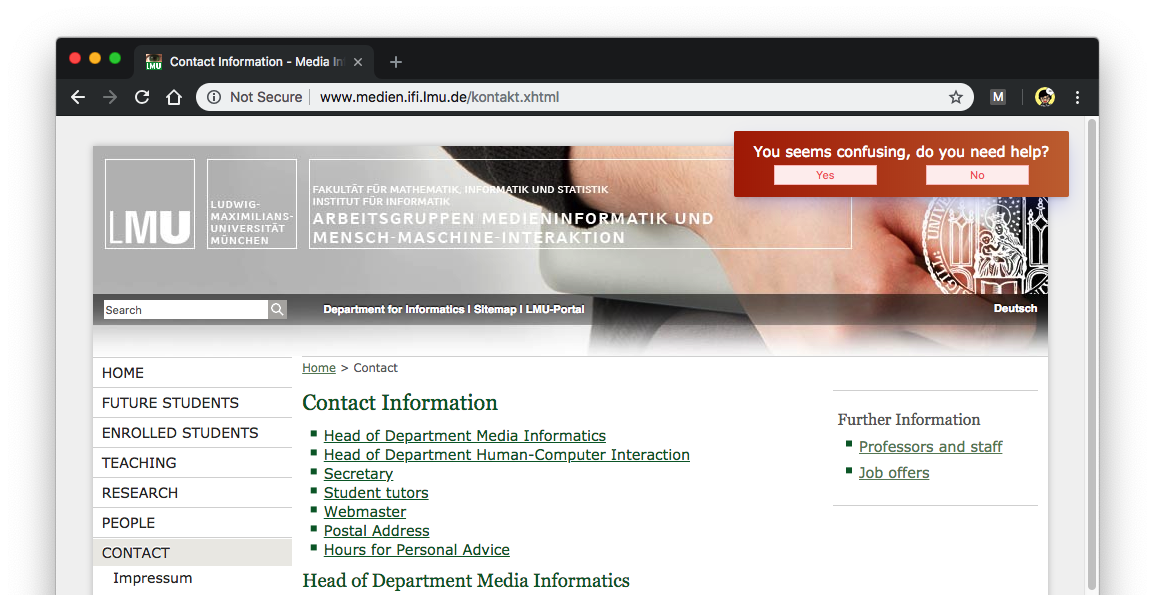
\includegraphics[width=0.7\textwidth]{figures/proactive-noti}
    \caption{TODO:}
    \label{fig:proactive-noti}
\end{figure}


\begin{figure}[H]
    \centering
    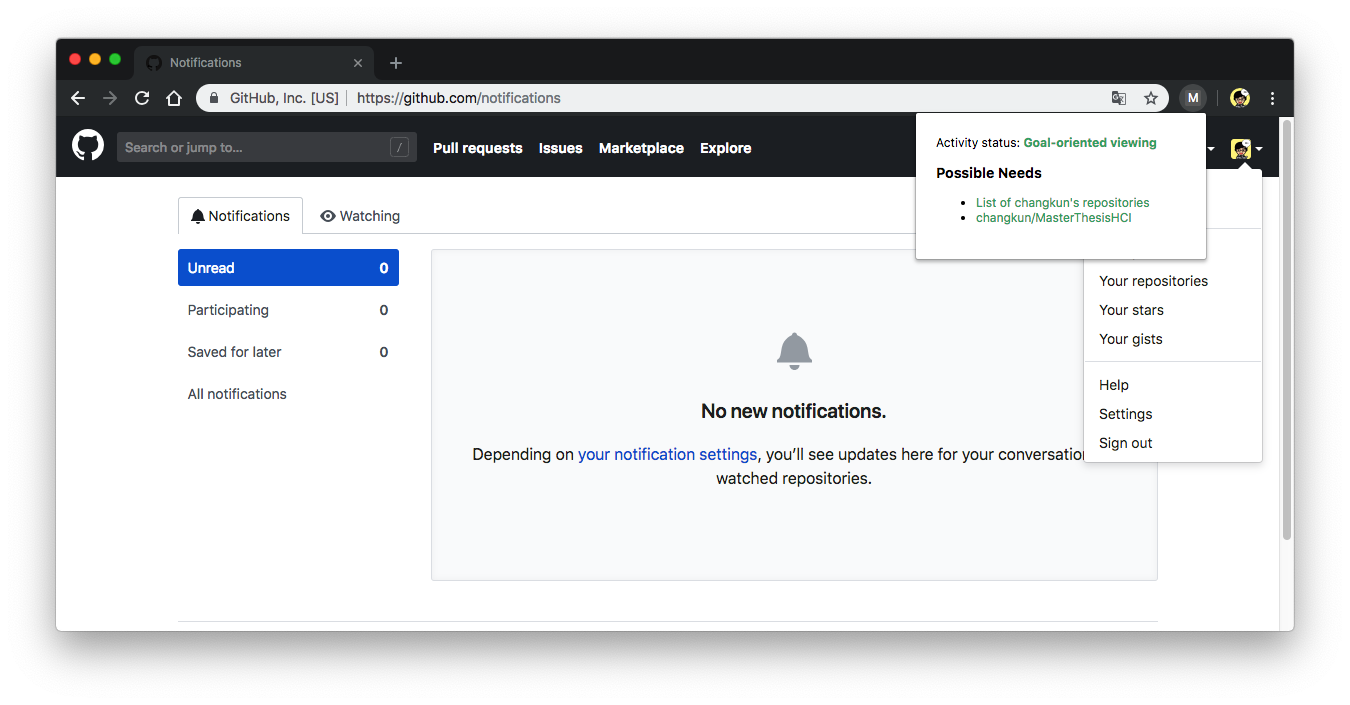
\includegraphics[width=0.7\textwidth]{figures/plugin-predicting-result}
    \caption{TODO:}
    \label{fig:plugin-predict}
\end{figure}

\begin{figure}[H]
    \centering
    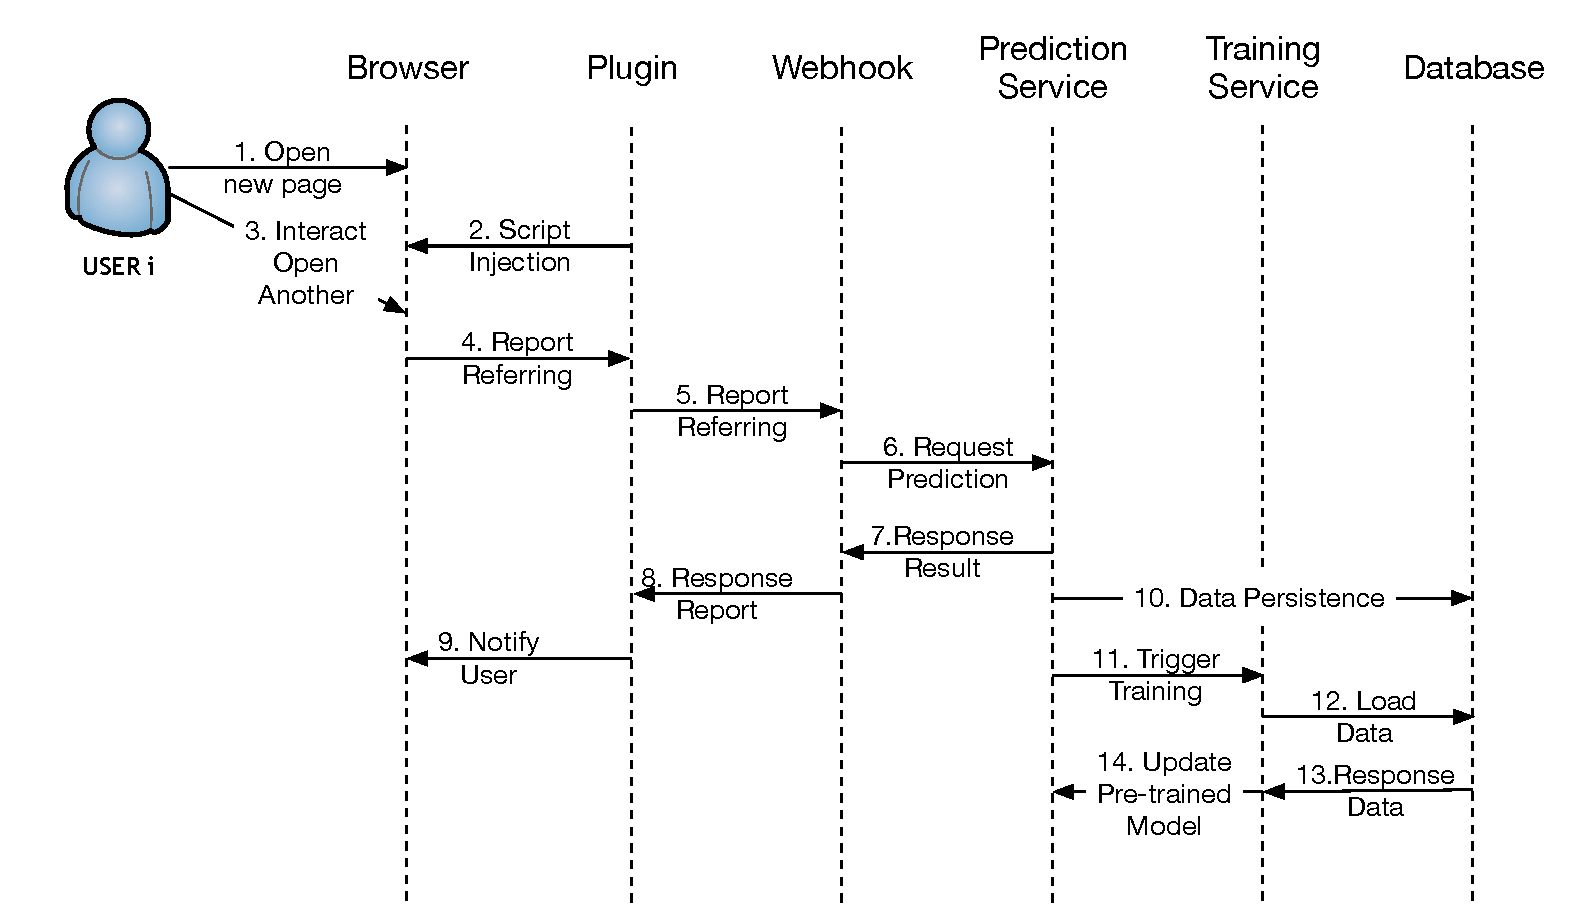
\includegraphics[width=0.7\textwidth]{figures/arch}
    \caption{TODO:}
    \label{fig:arch}
\end{figure}

\subsection{Standard Browser Web APIs}

Web APIs is a generic term used in various fields of development.
Web APIs in a context of web browsers mainly indicates the APIs provided
by browser manufactures to developers that helps web application can even close
to manipulate hardwares, for instance, WebAssembly \cite{w3c2018ws}.

Nowadays, there are experimental standard Web APIs integrates complex features to web developers, e.g. Web Speech APIs \cite{mozilla2019speech}, and only Google Chrome (after version 24) supports. The specification proposal was initiated by Google and according to the source code of Chromium, the APIs are implemented based on the speech recognition service provided by Google Cloud Platform \footnote{\url{https://github.com/chromium/chromium/blob/83928864c18362a4b0f84bad9bee4104f4655430/content/browser/speech/speech\_recognition\_engine.cc\#L35}, last accessed on January 03, 2019}.

\begin{figure}[H]
    \centering
    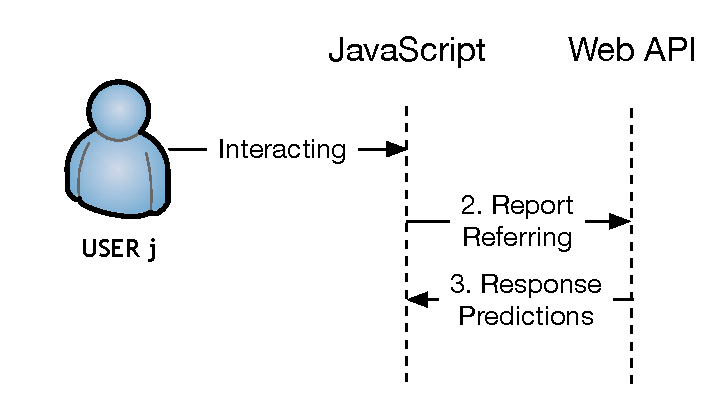
\includegraphics[width=0.4\textwidth]{figures/webapi}
    \caption{TODO:}
    \label{fig:webapi}
\end{figure}

% \subsubsection{Communication Protocol}

\cleardoublepage